\documentclass[conference]{IEEEtran}

%%%% Bibtex then pdfLatex

\usepackage{cite}
\usepackage{graphicx}
\usepackage{hyperref}
\usepackage{listings}
\usepackage{times}
\usepackage{xspace}
\usepackage{booktabs}
\usepackage{subfigure}
\usepackage{fancybox}
\usepackage{color}
\usepackage{multirow}
\usepackage{array}
%\usepackage{flushend}
\usepackage{subfigure}
\usepackage{balance} 
\usepackage{tabularx}
\newcommand{\todo}[1]{\colorbox{yellow}{\textbf{[#1]}}}
\newcommand{\emad}[1]{\textcolor{red}{{\it [Emad says: #1]}}}
\newcommand{\dan}[1]{\textcolor{blue}{{\it [Dan says: #1]}}}
\newcommand{\feedback}[1]{\textcolor{green}{{\it [Feedback says: #1]}}}

\hyphenation{op-tical net-works semi-conduc-tor}


\begin{document}



\title{CCCD: Concolic Code Clone Detection}

\author{\IEEEauthorblockN{Daniel E. Krutz and Emad Shihab}
Rochester Institute of Technology, USA\\
\{dxkvse,emad.shihab\}@rit.edu
}
\maketitle
\begin{abstract}


Code clones are multiple code fragments that produce similar results when provided the same input. Prior research has shown that clones can be harmful since they elevate maintenance costs, increase the number of bugs caused by inconsistent changes to cloned code and may decrease programmer comprehensibility due to the increased size of the code base.  

To assist in the detection of code clones, we propose a new tool known as Concolic Code Clone Discovery (CCCD). CCCD is the first known clone detection tool that uses concolic analysis as its primary component and is one of only three known techniques which are able to reliably detect the most complicated kind of clones, type-4 clones.


\end{abstract}


\IEEEpeerreviewmaketitle

\section{Introduction}

% Check to see if one of these citations may be removed


Code clones may adversely affect the software development process for several reasons. Clones often raise the maintenance costs of a software project since alterations may need to be done several times~\cite{Juergens:2009:CCM:1555001.1555062}. Additionally, unintentionally making inconsistent bug fixes to cloned code across a software system is also likely to lead to further system faults~\cite{Deissenboeck_2010}. 

There are four types of code clones which are generally recognized. Type-1 clones are the simplest and represent identical code except for variations in whitespace, comments and layout. Type-2 clones are syntactically similar except for variations in identifiers and types. Type-3 clones are two segments which differ due to altered or removed statements. Type-4 clones are the most difficult to detect and represent two code segments which significantly differ syntactically, but produce identical results when executed~\cite{Gold:2010:ICC:1808901.1808916}. 

In this paper, we propose Concolic Code Clone Detection (CCCD), a tool which uses~\emph{concolic analysis} as a driving force for discovering clones. Concolic analysis combines concrete and symbolic values in order to traverse all possible paths (up to a given length) of an application~\cite{Kim:2012:IAC:2337223.2337373}. CCCD is innovative for several reasons. First, only two other works~\cite{Kim:2011:MMC:1985793.1985835}~\cite{Kraw2012} are able to effectively discover type-4 clones. Additionally, it represents the only known proposed technique for discovering clones which is based on concolic analysis.

Concolic analysis assists in creating a powerful clone detection tool because it does not consider the syntactic properties of the source code of an application. Only the functionality is analyzed. This means that issues such as naming conventions and comments which have proven to be problematic for existing clone detection systems will have no adverse affect on CCCD.

\section{Tool Overview}
\label{sec: tooloverview}

Figure~\ref{fig:cccdstructure} shows the basic components of CCCD. As shown, CCCD is comprised of two primary phases. The first step is to generate the necessary concolic output for analysis and is accomplished using two components which are invoked from a Unix bash script. The first component is an open source tool for generating the concolic output known as CREST~\cite{Burnim:2008:HSD:1642931.1642995}. CREST was selected since it was able  to analyze a variety of function types, regardless of the signature. The second major component of the bash script is CTAGS~\footnote{http://ctags.sourceforge.net} which is used to identify the functions in the source code of the target application. 

The only modification which is done to CREST is with how it generates the necessary concolic output. Other than this, all default values are used and CREST is used in its native form. No details regarding the maximum path exploration length, main function for exploration or any other application details are needed. Only C programs are compatible with CCCD since CREST is only capable of analyzing C code.

The analysis phase is conducted using a component written in Java. This component separates the generated concolic output into individual function files using the list of functions generated by CTAGS as a guideline. Since the concolic output is separated at the function level, only function level clones are identified by CCCD. Code segments within functions or clones which partially traverse multiple functions will likely not be identified by CCCD.

Once the concolic information has been split into individual function files, the comparison process may begin. The concolic output for each function is compared to one another in a round robin fashion using the Levenshtein distance algorithm. Comparisons with a lower Levenshtein distance means the concolic output is more closely related, and thus indicative of a code clone candidate. The final report contains a listing of all code clone candidates as identified by CCCD.

\begin{figure}[thb!]
\vspace{2mm}
\centering
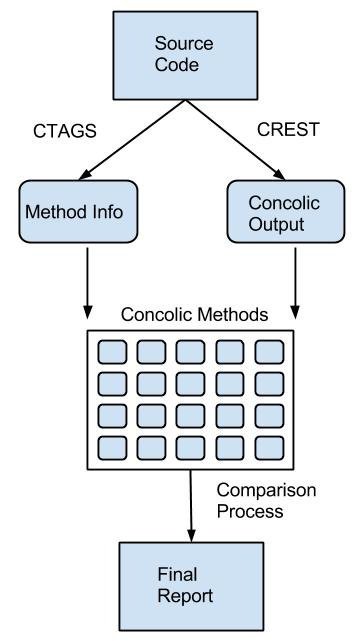
\includegraphics[width=33mm,height=60mm]{images/CCCDStructure_2.jpg}
\caption{Overview of the CCCD Tool}
\label{fig:cccdstructure}
\end{figure}


The tool and complete results may be found by visiting the main project website at \url{http://www.se.rit.edu/\~dkrutz/CCCD/}.


\section{Evaluation}
\label{sec: evaluation}


In order to evaluate CCCD, we first compare its performance on the code clone benchmarks provided by Krawitz~\cite{Kraw2012} and Roy~\emph{et al.}~\cite{Roy:2009:CEC:1530898.1531101}. These works provided several explicit examples of all four types of clones. The initial step was to ensure that CCCD would be able to detect all of these predefined clones individually. A simple C application was created which contained the sixteen clones as defined by Roy~\emph{et al.} and four as defined by Krawitz. 

Several functions were inserted into this class which were not clones of any other functions. The purpose of this was to help ensure that CCCD did not incorrectly identify functions to be clones which were not. This class was then analyzed by CCCD. Out of 465 comparisons, 296 were manually determined not to be comparisons between two functions which represented clones while 165 comparisons were manually determined to represent code clones. CCCD was then run against the target source code. Comparisons with a Levenshtein similarity score of under 35 were deemed to be code clone candidates. These values were selected after several previous test runs with this source code, along with the source code from other applications. Higher Levenshtein scores were found to include too many false positives, while lower scores ignored a large number of clones. All results were manually verified by two researchers.

CCCD was able to determine whether or not two functions were clones with an accuracy of 93\%. An additional, 17 comparisons were recommended for further manual analysis (i.e., had a Levenshtein score close to 35). Another 14 comparisons should have been identified as clones, but were not. These all interact with~\emph{Krawitz\_type4} clones. This is due to CREST's inability to traverse all paths of the code, thus creating incomplete concolic output and therefore hindering the ability of CCCD to detect clones. Since CCCD was able to identify the remaining type-4 clones presented in the work by Roy~\emph{et al.}, this is not considered to be a concern for CCCD. There were not false positives, meaning that all clone candidates identified by CCCD were manually verified to be actual clones. These results are shown in Table~\ref{table:completeKrawresults}.

% ``Not a Clone''


\begin{table}[thb!]
\begin{center}
\caption{Clone Detection Results}
    \begin{tabular}{ l | l }
    \toprule
 	Total Comparisons & 465 \\ \hline
	Not clones & 296 (65\%) \\ \hline
	Clones & 165  (35\%)  \\ \hline
	Correctly Identified & 434 (93\%) \\ \hline
	Not Identified & 14  (3\%) \\ \hline
	Recommended & 17  (3.5\%) \\ \hline
	False Positive & 0  (0\%) \\ \hline
	Avg. Leven Clones & 12.7 \\ \hline
	Avg. Leven Non-Clones & 58.4 \\ \bottomrule

    \end{tabular}
    
\label{table:completeKrawresults}
    \vspace{-0.2in}
\end{center}



\end{table}

The next step was to ensure that these clones could be discovered in several open source applications. These included FileZilla \footnote{https://filezilla-project.org}, VLC \footnote{http://www.videolan.org} and MySQL \footnote{http://www.mysql.com}. Each of the predefined clones taken from the works of Roy~\emph{et al.} and Krawitz were randomly inserted into the source code of these applications with their locations being noted. These results are shown in Table~\ref{table:injectedclones}.

\begin{table}[thb!]
\begin{center}
\label{table:injectedclones}
\caption{Results of the Injected Clones by CCCD}
    \begin{tabular}{ r | l | l | l | l | l }
    \toprule
    Application & Type-1 & Type-2 & Type-3 & Type-4 & Total \\ \hline\hline
    	VLC  & 5/5  &6/6   & 7/7  & 6/8  & 24/26 (92\%)\\ \hline
	MySQL & 5/5  &6/6   & 7/7  & 6/8  & 24/26 (92\%)\\ \hline
	FileZilla & 5/5  &6/6   & 7/7  & 6/8  & 24/26 (92\%)\\ \bottomrule
    \end{tabular}
\end{center}
%\vspace{-0.3in}
\vspace{2mm}
\end{table}



\section{Conclusion and Future Work}
\label{sec: conclusion}

This paper presented CCCD, a tool which uses concolic analysis to discover code clones. Preliminary work demonstrated its effectiveness in discovering clones of all four types. This includes type-4 clones, which only two other techniques are able to reliably locate. 





%\vspace{-0.2in}
\bibliographystyle{plain}
\bibliography{refs}

\end{document}






